% ---------
%  Compile with "pdflatex hw0".  
% --------
%!TEX TS-program = pdflatex

\documentclass[letterpaper,11pt]{article}
\usepackage{jeffe,handout,graphicx}
\usepackage{fancyhdr}
\usepackage{comment}
\graphicspath{{./Fig/}}

\bibliographystyle{unsrt}
% ---------
% Input file uses Unicode's UTF-8 encoding
% ---------
%!TEX encoding = UTF-8 Unicode
\usepackage[T1]{fontenc}
\usepackage[utf8]{inputenc}

% ---------
%  The next several lines (up to the line of =='s) change the default text
%  and math fonts and make a few other minor cosmetic changes.  If you get
%  any error messages related to these packages, just comment them out.
%         -- Jeff
% --------
\usepackage[charter]{mathdesign}
 \def\sfdefault{fvs}
 \def\ttdefault{fvm}
 \SetMathAlphabet{\mathsf}{bold}{\encodingdefault}{\sfdefault}{b}{\updefault}
 \SetMathAlphabet{\mathtt}{bold}{\encodingdefault}{\ttdefault}{b}{\updefault}
 \SetMathAlphabet{\mathsf}{normal}{\encodingdefault}{\sfdefault}{\mddefault}{\updefault}
 \SetMathAlphabet{\mathtt}{normal}{\encodingdefault}{\ttdefault}{\mddefault}{\updefault}
 \usepackage{microtype}
% ---------
%  End of cosmetics.
% --------

\newcommand{\name}{Zigang Xiao (zxiao2), Yuelin Du (du6), Pei-Ci Wu (peiciwu1)} 
\newcommand{\hwnumber}{5}                % fill homework count
\newcounter{probid}
\newtheorem{definition}{Definition}
\newtheorem{theorem}{Theorem}
\newcommand{\hdr}[2]{
   \newpage\setcounter{page}{1}       % reset page counter
   \lhead{\fancyplain{}{\textbf{#1}}}
   \rhead{\fancyplain{}{\textbf{#2}}}
   \cfoot{\fancyplain{}{\thepage}}
}

\newcommand{\stmt}{
 \EMPH{I understand the course policies.}
}

\newcommand{\saystmt}{
($\bullet$) \EMPH{I understand the course policies.}
}

\newcommand{\newprob}{
\hdr{CS 573 HW\hwnumber}{\name{} HW\hwnumber{} \#\arabic{probid}}
\stepcounter{probid}
\item
}

% =========================================================
\begin{document}
\pagestyle{fancy}
\fancyhf{}
\small\sf	% typeset excetps from problems in a different, smaller font

\begin{enumerate}
% ---------------------------------------------------------
\newprob
\saystmt

Describe and analyze an algorithm to nest the boxes so that the number of
visible boxes is as small as possible.

\begin{solution}
  We assume one box can only contain \emph{exactly} one another box.
  We reduce this problem to bipartite matching problem, and then 
  use Ford-Fulkerson algorithm to solve it.
  We construct a bipartite graph $G$ with vertex set $U \cup W$ as follows:
  \begin{itemize}
    \item Each box is a node in both $U$ and $W$.
    \item For a pair of node $u\in U$ and $v \in W$, if $u$ can be rotated so 
      that it can be contained in $v$, we add an edge $e=(u,v)$.
  \end{itemize}

  Call two boxes are nested if one contains another.
  Let $N$ be the maximum number of nested boxes.
  Then, the number of visible boxes can be simply computed as $n-N$.

  \begin{theorem}
    The maximum number of nested boxes equals to $|M|$, where $|M|$ is the
    value of the size of the maximum matching in $G$.
  \end{theorem}

  \begin{proof}
    If we know the maximum number of nested boxes and how the boxes contain
    each other, we can transfer to a maximum matching in $G$ as follows: 
    if $u$ contains $v$, then we select $e=(u,v)$ in $G$, where $u\in U$ and
    $v\in W$.  Each time we place a box into another, the number of visible
    boxes is decreased by one.  
    Let $|M|$ be the final number of edges selected.
    It is maximized according to the above procedure.
    Otherwise, there will be a better way to place the boxes. 
    Since each box can contain exactly one another box, this is a valid
    matching.  Moreover, the number of the nested boxes and the size of the
    maximum matching is $|M|$. 

    Conversely, if we know a maximum matching, we can find how to place the
    boxes into each other and then get the smallest number of visible boxes.
    If we match $u$ with $v$, then we place box $u$ into $v$.
    Finally, the size of the maximum matching is $|M|$, and equals to the
    number of nested boxes. 
  \end{proof}

  There are at most six permutation of width, height and depth. Hence for a
  pair of boxes, we can determine whether they can contain one another in
  constant time. Let there be $n$ boxes. Then, there are $2n$ nodes and at most
  $O(n^2)$ edges in $G$.  Hence, the maximum flow has value at most $O(n)$, and
  the Ford-Fulkerson algorithm runs in $O(n^3)$ time.

\end{solution}

% ---------------------------------------------------------
\newprob
\saystmt

Describe an efficient algorithm that either rounds $A$ in this fashion, or
reports correctly that no such rounding is possible.

\begin{solution}
  We can solve this problem by reducing it to maximum flows problem 
  with edge demands.
  Before we do that, 
  we first check if the sum of each row (or column)
  is an integer. If not, we report that no such rounding is possible. 
  This is because after rounding, the sum of each row (or column) must be an
  integer.
  
  Now we assume the sum of each row (or column) is an integer.
  Let $R[1..m]$ be the sum of each row, and $C[1..n]$ be the sum of each column.
  We construct a graph $G$ with vertex set $\{s,t\} \cup U \cup V \cup W$ as follows:
  \begin{itemize}
    \item Each element $A[i][j]$ is a node $x_{ij}$ in $U$.
    \item Each row $i$  is a node $r_i$ in $V$.
    \item Each column $j$  is a node $c_i$ in $W$.
  \end{itemize}

  The edges consists of:
  \begin{itemize}
    \item an edge $e: s \rightarrow x_{ij}$ with capacity $c(e)=\lceil x_{ij}
      \rceil$ and demand $d(e) = \lfloor x_{ij} \rfloor$ for each $x_{ij} \in U$.  
    \item an edge $e: x_{ij}\rightarrow r_i$ with capacity $c(e)=\infty$ and
      demand $d(e)=0$ for each $r_i \in V$.
    \item
      an edge $e: x_{ij} \rightarrow c_j$ with capacity $c(e)=\infty$ and
      demand $d(e)=0$ for each $c_i \in W$.
    \item an edge $e: r_i \rightarrow t$ with capacity $c(e)=d(e)=R[i]$ 
      for each $r_i \in V$.
    \item an edge $e: c_j \rightarrow t$ with capacity $c(e)=d(e)=C[j]$ 
      for each $c_j \in W$.
  \end{itemize} 

  \begin{theorem}
    The rounding exists if and only if there is a maximum flow that saturates
    every edge entering $t$. The rounding scheme consists of 
    the flow values that leave from $s$.
  \end{theorem}
  \begin{proof}
    If we know a correct rounding scheme, we can transform it to a feasible
    flow in $G$. For each $x_{ij}=A[i][j]$, we push the same amount of flow to
    edge $s \rightarrow x_{ij}$. Since $x_{ij}$ can only be rounded to $\lfloor
    x_{ij} \rfloor$ or $\lceil x_{ij} \rceil$, clearly the values satisfy the
    edge constraints of these edges.  Moreover, since this is a valid rouding
    scheme, the sum of rows and columns will be exactly the same as the flow
    value on edges $r_i \rightarrow t$ or $c_j \rightarrow t$, which means
    these edges are saturated and thus it is a maximum flow.

    Conversely, if we have a maximum flow that saturates every edge entering
    $t$, we can round each element $A[i][j]=f(e)$, where $e$ is the edge
    $s\rightarrow  x_{ij}$. The flow value $f(e)$ satisfies 
    $d(e) \leq f(e) \leq c(e)$. Thus, each entry $x_{ij}=A[i][j]$ is rounded
    correctly to $\lfloor x_{ij} \rfloor$ or $\lceil x_{ij} \rceil$.
    Finally, the sum of rows and columns are the same as the 
    corresponding capacity (or demand) values in edges $r_i \rightarrow t$ and 
    $c_j \rightarrow t$. Since all these edges are saturated, the sum of entries
    in any row or column are unchanged.
    Thus, it is a valid rounding scheme.
  \end{proof}

  Clearly, there are $O(mn)$ vertices  and $O(mn)$ edges in $G$.
  Computing the sums and constructing the graph can be done in $O(mn)$ time.
  If we use Edmonds-Karp fat-pipe algorithm, we get an overall running time of 
  $O(VE^2)=O(m^3n^3)$.
\end{solution}

% ---------------------------------------------------------
\newprob
\saystmt

Describe and analyze an algorithm to compute a donation schedule, describing
how much money each voter should send to each candidate on each day, that
guarantees that every candidate gets enough money to win their election.  The
schedule must obey both Federal laws and individual voters' budget constraints.
If no such schedule exists, your algorithm should report that fact.

\begin{solution}
  Suppose there are $k$ days left from now to the election, there are $c$
  candidates and $v$ voters.  Let $M[1..c]$ be the money that must be spent on
  each candidate, $W[1..v][1..c]$ be the amounts that each voter is willing to
  donate to each candidate $A[1..v]$ be the total amounts that each voter is
  able to donate to all candidates.
  We can model this problem as a maximum flow problem.
  We construct a flow network $G=(V,E)$ with vertices $X \cup Y \cup \{s,t\}$,
  where each node in $X$ and $Y$ denotes a voter and a candidate, respectively.
  The edges consist of:
  \begin{itemize}
    \item an edge $s \rightarrow x$ with capacity $\min\{100, A[x]/k\}$ for
      each $x\in X$.
    \item an edge $y \rightarrow t$ with capacity $M[y]/k$ for each $y \in Y$.
    \item an edge $x \rightarrow y$ with capacity $W[x][y]/k$ for each $x\in X$
      and $y \in Y$.
  \end{itemize}

  \begin{theorem}
    The donation schedule exists if and only if there is a maximum flow that 
    saturates every edge entering $t$. The money that each voter should spend
    to each candidate on every day is denoted by the edges $x \rightarrow y$
    for each $x\in X$ and $y \in Y$.
  \end{theorem}

  \begin{proof}
    For each edge $s \rightarrow x$ for each $x \in X$, clearly it satisfies
    both Federal lasw and individual voters' budget constraints.
    For each edges $x \rightarrow y$, it denotes the amount that voter $x$ 
    will send to candidate $y$ each day.
    For each edge $y \rightarrow t$ for each $y \in Y$, it denotes the amount 
    that every candidate must receive each day to meet the campaign
    requirement.
    If the maximum flow we compute saturates all the edges entering $t$,
    then following this schedule, after $k$ days each candidate can receive 
    exactly $M[y]$ money for all $y \in Y$.
    Hence, the maximum flow we compute is the desired schedule.
  \end{proof}

  The maximum flow has value at most $S=\sum_y M[y]$. There at most 
  $v + v \cdot c + c = O(vc)$ edges. Thus, Ford-Fulkerson algorithm
  runs in $O(Svc)$ time.
\end{solution}

% ---------------------------------------------------------
\newprob

\begin{enumerate}
  \item[($\bullet$)] \stmt
  \item 
Prove that this greedy strategy does not always compute an optimal solution.

\begin{solution}
  We prove by giving a counterexample. As in the following figure, 
  the blue cells are marked. Both of the 2-bend and 3-bend paths contains 
  maximum number of marked cells. However, if we choose the 2-bend path 
  at the first iteration, we need another two monotone path to cover all the
  cells. On the other hand, choosing the 3-bend path at first can finish 
  marking the cells with only two paths.
  \begin{center}
    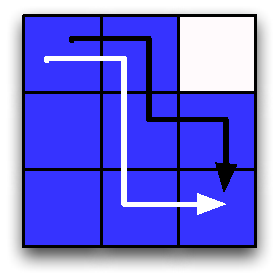
\includegraphics[width=.1\textheight]{p4}
  \end{center}
\end{solution}

\item
Describe and analyze an efficient algorithm to compute the smallest set of
monotone paths that covers every marked cell. The input to your algorithm is an
array $M[1..n,1..n]$ of booleans, where $M[i, j]$ = True if and only if cell
$(i, j)$ is marked.

\begin{solution}
  Dynamic programming to construct the graph $G$.
  Maximum flow with unit demand and cost on each edge.
  $d=1$ means each node must be used.
  $\$=1$ means the more paths are used, the more cost there will be,
  because all flows are sent from $s$.
  \begin{proof}
    Minimum set of monotone paths $\rightarrow$ minimum cost flow.
  \end{proof}
\end{solution}

\end{enumerate}


% ---------------------------------------------------------
\newprob

\begin{enumerate}
  \item[($\bullet$)] \stmt
  \item 
    Prove that if Paul uses a deterministic strategy, and Sally knows his
    strategy, then Sally can guarantee that she wins.
  \item 
    Describe a deterministic strategy for Sally that guarantees that she wins
    when $r \leq M$, no matter what strategy Paul uses.
  \item 
    Prove that if Sally uses a deterministic strategy, and Paul knows her
    strategy then Paul can guarantee that he wins when $r < M$.
  \item 
    Describe a randomized strategy for Sally that guarantees that she wins with
    probability at least $\min{r/M,1}$, no matter what strategy Paul uses.
  \item 
    Describe a randomized strategy for Paul that guarantees that he loses with
    probability at most $\min{r/M,1}$, no matter what strategy Sally uses.

\end{enumerate}

% =========================================================

\end{enumerate}
\end{document}
